%%%%%%%%%%%%%%%%%%%%%%%%%%%%%%%%%%%%%%%%%%%%%%%%%%%%%%%%%%%%%%%
%
% Welcome to Overleaf --- just edit your LaTeX on the left,
% and we'll compile it for you on the right. If you open the
% 'Share' menu, you can invite other users to edit at the same
% time. See www.overleaf.com/learn for more info. Enjoy!
%
%%%%%%%%%%%%%%%%%%%%%%%%%%%%%%%%%%%%%%%%%%%%%%%%%%%%%%%%%%%%%%%
\documentclass{beamer}
\usepackage{tikz}
\usetheme{Madrid}
\usepackage{ctex}
\usecolortheme{default}
\usepackage{verbatim}
\title[2022.11.21日汇报] %optional
{2022.11.21汇报}
%\subtitle{Demonstrating the Berkeley theme}
\author[周添文] % (optional)
{周添文\inst{} }

\institute[] % (optional)
{
  \inst{}%
  数学科学学院\\
  北京师范大学\\
 % \and
  %\inst{2}%
%  Faculty of Chemistry\\
%  Very Famous University
}

\date[2022.11.21] % (optional)
%{Very Large Conference, April 2021}

% Use a simple TikZ graphic to show where the logo is positioned

%\node[draw,color=white] at (0,0) {LOGO HERE};


%End of title page configuration block
%------------------------------------------------------------
%The next block of commands puts the table of contents at the 
%beginning of each section and highlights the current section:

\AtBeginSection[]
{
  \begin{frame}
    \frametitle{Table of Contents}
    \tableofcontents[currentsection]
  \end{frame}
}
%------------------------------------------------------------
\begin{document}
\frame{\titlepage}
%\logo{\includegraphics[]{bnu.png}}
%---------------------------------------------------------
%Highlighting text
\begin{frame}
\frametitle{耀斑(Flare)类杂散光的自动探测与去除方法}

\begin{itemize}
\item 耀斑类杂散光的自动探测
\item 光源检测
\item 耀斑检测
\item 耀斑位置的确定方法
\item 耀斑去除
\end{itemize}
%\begin{comment}
%\begin{block}{Remark}
%Sample text
%\end{block}

%\begin{alertblock}{Important theorem}
%Sample text in red box
%\end{alertblock}

%\begin{examples}
%Sample text in green box. The title of the block %is ``Examples".\pause

%HI

%\end{examples}
\end{frame}
\begin{frame}
\frametitle{光源检测}
%\begin{itemize}
%\item 

由文献[1]可知,耀斑伪影(flare artifact)一般产生在光源对面的对称点处。\pause


设$u:\Omega \rightarrow \mathbb{R}^3$为一个图像,其中$\Omega \subset \mathbb{R}^2$代表图像的定义域(domain),则我们可以按照下述方法找到耀斑伪影的位置:找到穿过光源和\textbf{主点}(principal point)的线,在定义域中找到靠近这条直线的点。\pause


主点指的是\textbf{主光轴}(principal axis)和像平面的交点。在此处,我们大致地定义主点为定义域的中心,记作$x_c$。
\end{frame}
\begin{frame}
\frametitle{光源检测}
接下来,我们需要确定定义域中的亮光源${x_S}_i,i=1,...,s,$进而确定图像中耀斑的位置。\pause


考察在CIELab色彩空间下的图像$u^{La*b*}=u^L,u^{a*},u^{b*}:\Omega \rightarrow \mathbb{R}^3$,其中的$u^L(x)$代表着$x\in \Omega$处的亮度(Luminance)。\pause

CIELab 颜色空间(Lab color space)是在1976年出现的。这种颜色空间包括人眼所能看到的所有颜色(可见光谱),所以也是目前为止色域最宽的颜色空间,其每一组色值对应一种确定的与设备无关的色彩。\pause
\end{frame}
\begin{frame}
\frametitle{CIELab色彩空间}
在Lab颜色空间中,一种颜色由L(明度),a*颜色,b*颜色三个参数表示;在一幅图像中,每一个像素对应一个Lab值,L,a*,b*三个参数的取值范围如下所述。\pause


L:取值范围为$[0, 100]$,表示纯黑色到纯白色范围;

a:取值范围为$[-128, 127]$,表示绿色到杨红色范围;

b:取值范围为$[-128, 127]$,表示蓝色到黄色范围。

\end{frame}
\begin{frame}
\frametitle{光源检测}
因此,为了找到亮度最大的区域,我们需要我们需要$u^L$更加接近100。由此,我们考察$u^L$的\textbf{上水平集}(upper level set)
\begin{equation}
X_lu^L:=\{u^L\geq l\}=\{x\in \Omega:u^L(x)\geq l\}.
\end{equation}\pause

其可以写作有穷多个联通分支(connected components)的并集,我们选取其中面积最大的联通分支$S_1$,其即为主光源。\pause


除此以外,我们选取面积大于等于$0.8\times S_1$的所有联通分支,记为$S_i$,并近似地将他们的重心当作近似的中心,记为${x_S}_i$
\begin{equation}
{x_S}_i=\frac{1}{area(S_i)}\sum_{x\in S_i}x,x\in \Omega
\end{equation}
\end{frame}
\begin{frame}
\frametitle{耀斑检测}
 为了更合理地检测耀斑位置,我们需要进行如下假设:
 \begin{itemize}
 \item 耀斑是图像$u$中的一个\textbf{明亮斑点}(bright blob)\footnote{一个斑点(blob)可以看作图像中比背景更亮或更暗的区域,并且由平滑弯曲的边界所包围},我们通常用\textbf{关键点}$x_k$代表一个耀斑。\pause
 \item 由于耀斑一般具有圆形或椭圆形形状,因此上述明亮斑点不应太过细长\pause
 \item 耀斑的大小有限,是有界限的\pause
 \item 由Rayleigh公式,耀斑的CIELab颜色应当有较高的L值和负的a*值\pause
 
 \end{itemize}
\end{frame}
\begin{frame}
\frametitle{明亮斑点检测}
首先,我们按照前文中的规定,将耀斑定义为比背景更亮的明亮斑点(blob)。根据文献[3]中描述,我们将关键点$x_k\in \Omega \subset \mathbb{R}$定义为方程
\begin{equation}
L(x,\sigma)=G(x;\sigma)\ast u^g(x)
\end{equation}
的局部极大值。\pause

其中,$\ast $是$\mathbb{R}^2$中的卷积(convolution),$u^g$是图像$u$的灰化版本(仅保留$u^L$)。$G(x;\sigma)$是各向同性(isotropic)的归一化高斯函数,标准差为$\sigma$,其在全平面上积分为1.$L(x,\sigma)$是平面上的Laplace算子,
\begin{equation}
\Delta L=\frac{\partial^2 L}{\partial x^2}+\frac{\partial^2 L}{\partial y^2}
\end{equation}
\end{frame}
\begin{frame}
\frametitle{明亮斑点检测}
我们考察DOG(the Difference Of Gaussian)
\begin{equation}
D(x,\sigma)=L(x,k\sigma)-L(x,\sigma),k\in \mathbb{R}
\end{equation}\pause
其可以近似估计正规化的Laplace算子$
\sigma^2\Delta L(x,\sigma)$.在本算法中,由于我们的假设,可以得知耀斑位于$D(x,\sigma)$的最小值处.
\end{frame}
\begin{frame}
\frametitle{耀斑的边界}

由前假设,我们知道耀斑是有界的。假设$x_k(j)$为一个关键点,我们考察和其亮度相似的像素点的全体,其中$\delta$为邻域半径:
\begin{equation}
B_{\delta}(x_k(j))=\{x\in \Omega: |u^L(x_k(j))-u^L(x)|\leq \delta\}
\end{equation}\pause

设$cc(B_{\delta}(x_k(j));x_k(j))$是$B_{\delta}(x_k(j))$包含关键点$x_k(j)$的连通分支,则该连通分支内包含着所有与$x_k(j)$亮度相似的点。我们规定,上述连通分支的面积应该小于整体光源面积的1\%,即
\begin{equation}
area(cc(B_{\delta}(x_k(j));x_k(j)))<\frac{area(S)}{100}
\end{equation}
\end{frame}
\begin{frame}
\frametitle{去除细长型明亮斑点}
由前假设,耀斑只有近似圆形的形状,由文献[4]中方法,我们可以计算$D=L(x,k\sigma)-L(x,\sigma)$的Hessian矩阵特征值$\lambda_1,\lambda_2$. \pause
由于关键点$x_k(j)$是$D$的最小值,故由矩阵论,可知$\lambda_1,\lambda_2\geq 0$. \pause

进一步来说,$\lambda_1,\lambda_2$需要满足下述条件:
\begin{equation}
{\lambda}_1>0,{\lambda}_2<4{\lambda}_1
\end{equation}
其保证了D的确取到了最小值,同时并不是细长型斑点。\end{frame}
\begin{frame}
\frametitle{耀斑位置的确定方法}
我们将引入如下几种判别方法,判断明亮斑点确为耀斑的可能性:

1.关键点的位置
\begin{itemize}
\item 从关键点$x_k(j)$到图像中心$x_c$的距离与从光源$x_s$到图像中心$x_c$的距离相似\pause

\item 记光源$x_s$和图像中心$x_c$的连线为$l$,$x_k(j)$到$l$的距离足够小\pause
\end{itemize}
2.La*b*的值
\begin{itemize}
\item $u^L$较大
\item $u^a$为负
\item$u^b$无限制\pause
\end{itemize}
接下来,我们将利用上述方法,阐述耀斑去除的过程:
\end{frame}
\begin{frame}
\frametitle{建立掩膜}
\textbf{掩膜}(Mask)是图像处理中的常用工具。我们用到的是\textbf{二元掩膜}(Binary Mask),在图像处理中,计算机将图像识别为矩阵,而掩膜同样为一个矩阵,其在希望过滤掉的部分值为0,其他部分值为1,以此达成\textbf{过滤图像信息}的目的。\pause

通常来说,(二元)掩膜具有如下应用:
\begin{itemize}
\item 提取感兴趣区:用预先制作的感兴趣区掩膜与待处理图像相乘,得到感兴趣区图像,感兴趣区内图像值保持不变,而区外图像值都为0;\pause
\item 屏蔽作用:用掩膜对图像上某些区域作屏蔽,使其不参加处理或不参加处理参数的计算,或仅对屏蔽区作处理或统计;\pause
\item 结构特征提取:用相似性变量或图像匹配方法检测和提取图像中与掩膜相似的结构特征;
\end{itemize}
\end{frame}

\begin{frame}
\frametitle{建立掩膜}
在此问题中,我们先考察耀斑对图像像素的影响,其分为以下几步:\pause
\begin{itemize}
\item 给定$\delta>0$,考虑$B_{\delta}(x_
{fs})=\{x\in \Omega: |u^L(x_k(j))-u^L(x)|\leq \delta\}$,取定其中包含关键点$x_{fs}$的连通分支,记作$C_{\delta}(x_{fs})$\pause
\item 取$C_{\delta}(x_{fs})$半径为$\epsilon>0$的扩张(dilation)$C_{\delta}^{\epsilon}(x_{fs})$,注意这一扩张中可能包含并不在连通分支中的点\pause
\item 给定$\omega$为图像内的其他像素,为了减小计算量,将$u^L(x)$进行标准化,表达为
\begin{equation}
u^L_{norm}(x)=\frac{u^L(x)-min(u^L,\omega)}{max(u^L,\omega)-min(u^L,\omega)}
\end{equation}
使得$u^L_{norm}(x)$在0到1内取值
\end{itemize}
\end{frame}
\begin{frame}
\frametitle{建立掩膜}
最终,耀斑区域可以写为:
\begin{equation}
F(x_{fs})=C_{\delta}^{\epsilon}(x_{fs})\cap x_{\alpha}u^L_{norm}
\end{equation}\pause
其中,$x_{\alpha}u^L_{norm}$代表水平集$[u^L_{norm}\geq \alpha]$,$\alpha$由试验确定为0.2.\pause

掩膜矩阵$M:\Omega \rightarrow \mathbb{R}$的表达式为:
\begin{equation}
M(x)=1, x\in F(x_{fs})
\end{equation}
 其余情况下,$M(x)=0$
\end{frame}
\begin{frame}
\frametitle{耀斑去除}
为了能够重建被耀斑损坏的区域$O\subset \Omega\subset \mathbb{R}^2$,可以将其视作寻找$x\in O$在映射$\phi:O\rightarrow O^c$下的像$\phi(x)$的过程\pause
而在$O^c$中,像的情况是已知的,只需要求解如下能量方程:\pause
\begin{equation}
\epsilon_{E}(\hat{u},\phi)=\int_{\hat{O}}E(p_{\hat{u}}(x)-p_{u}(\phi(x)))dx
\end{equation}
其中$O=\bigcup_{i=1}{s}F(x_{fs}^{i})$

\end{frame}
\begin{frame}
\frametitle{算法}
\begin{figure}[!h]
\centering
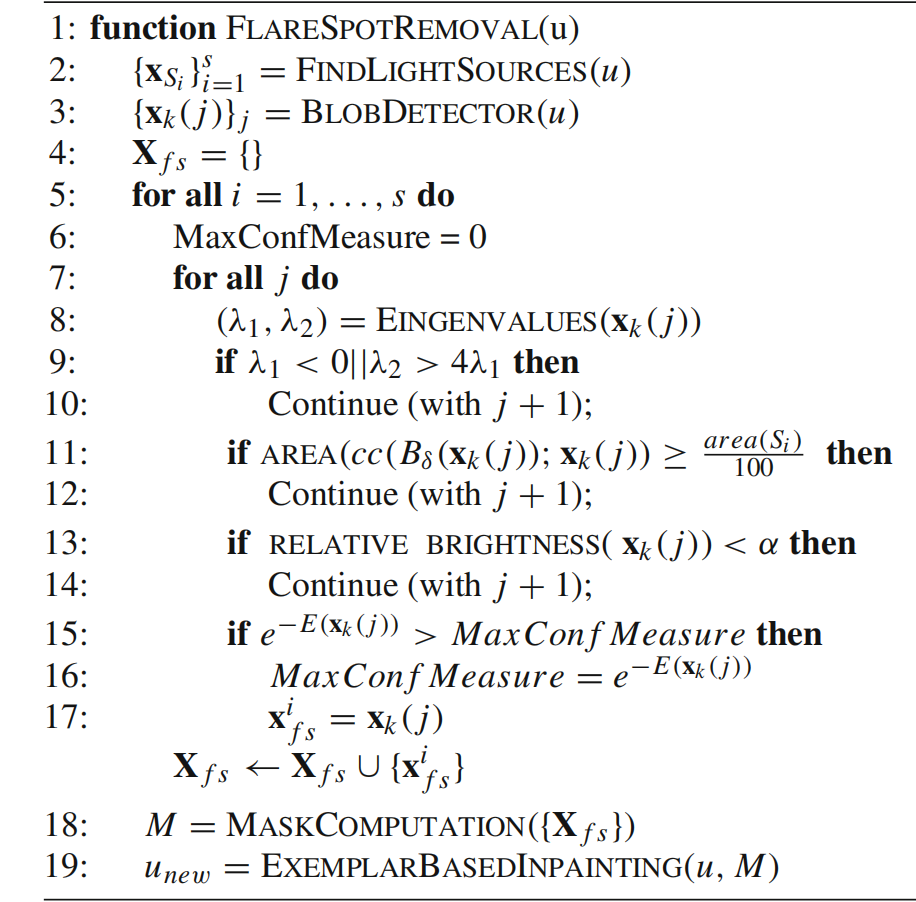
\includegraphics[height=8cm,width=8cm]{图片1.png}
\caption{算法示意图}
\end{figure}

\end{frame}
\begin{frame}
\frametitle{参考文献}
\begin{thebibliography}{99}
\bibitem{article1}
Evans, E. D.: An analysis and reduction of flare light in optical
systems. PhD thesis, The Ohio State University (1988)
\bibitem{article2}Vitoria P, Ballester C. Automatic flare spot artifact detection and removal in photographs[J]. Journal of Mathematical Imaging and Vision, 2019, 61(4): 515-533.
\bibitem{article3} Lowe, D.G.: Object recognition from local scale-invariant features.
In: The proceedings of the seventh IEEE international conference
on Computer vision, vol. 2, pp. 1150–1157. IEEE (1999)
\bibitem{article4}Lowe, D.G. Distinctive Image Features from Scale-Invariant Keypoints. International Journal of Computer Vision 60, 91–110 (2004). https://doi.org/10.1023/B:VISI.0000029664.99615.94
\end{thebibliography}
\end{frame}
\end{document}